\documentclass[a4paper]{report}
\usepackage[T1]{fontenc}
\usepackage[utf8]{inputenc}
\usepackage[english]{babel}
\usepackage{geometry}
\usepackage{graphicx}
\usepackage{subfig}
\geometry{a4paper,top=2.5cm,bottom=2.5cm,left=3cm,right=3cm,%
	heightrounded,bindingoffset=5mm}
\begin{document}

\title{\Huge{JustRecipe}}
\author{\Large{Francesco Campilongo - Daniele Cioffo - Francesco Iemma}}
\date{Academic Year 2020/21}
\maketitle
\tableofcontents

\chapter*{Introduction}

\chapter{Dataset}


\chapter{Design}
\section{Introduction To The Application}
The topic of cuisine is extensively widespread in our society. In fact we can think at the success achieved by tv shows related to cooking in the last years and also at the fact that a lot of chefs are becoming superstars.
Then there is another important factor: the coronavirus outbreak.

\noindent With the coronavirus outbreak a lot of people became cuisine lovers, in fact at the first moments of the pandemia several ingredients as flour and yeast were very hard to find, because people were confined in their home and so they had more free time.

\noindent But this topic is not a recente one. The first recipe book dates back to eigth century B.C. and it is the so-called \emph{Eraclio} (by the name of the city in which he was found). Then also an important latin writer, Apicio, wrote one of the most important recipe books of the roman era: \emph{De Re Coquinaria} which dates back to the first century B.C..
 
\noindent So the topic of cuisine is inherent to human nature, because the necessity of eating is a basic need.
Furthermore, everyone has experimented the infamous question: “What will I eat this evening?”. JustRecipe has the aim of answer to this question, it has the aim of helping university student or workers to retrieve and to do fast and simple recipes.

\noindent So this application is basically a recipe book but it is also more than this.

\noindent JustRecipe is also a social network which allow people to enjoy, to ex-change ideas about cooking, to feel less lonely in this hard period.

\section{Requirements}
\subsection{Main Actors}
\subsection{Functional Requirements}
Unregistered User
\begin{itemize}
	\item Sign-up
\end{itemize}
User
\begin{itemize}
	\item Login/Logout
	\item Search a recipe
	\item Browse suggested recipes
	\item Browse recipes of following users
	\item Add a recipe
	\item Edit own recipes
	\item Comment recipes
	\item Follow another user
	\item Like a recipe
\end{itemize}
Moderator
\begin{itemize}
	\item Delete comments
\end{itemize}
Administrator
\begin{itemize}
	\item Delete users
	\item Delete recipes
	\item Elect moderators
\end{itemize}
\subsection{Non-Functional Requirements}

\subsection{Actors and Use Cases}
The use case diagram of the application is described in the figure 2.1 
\begin{figure}[htpb]
	\centering
	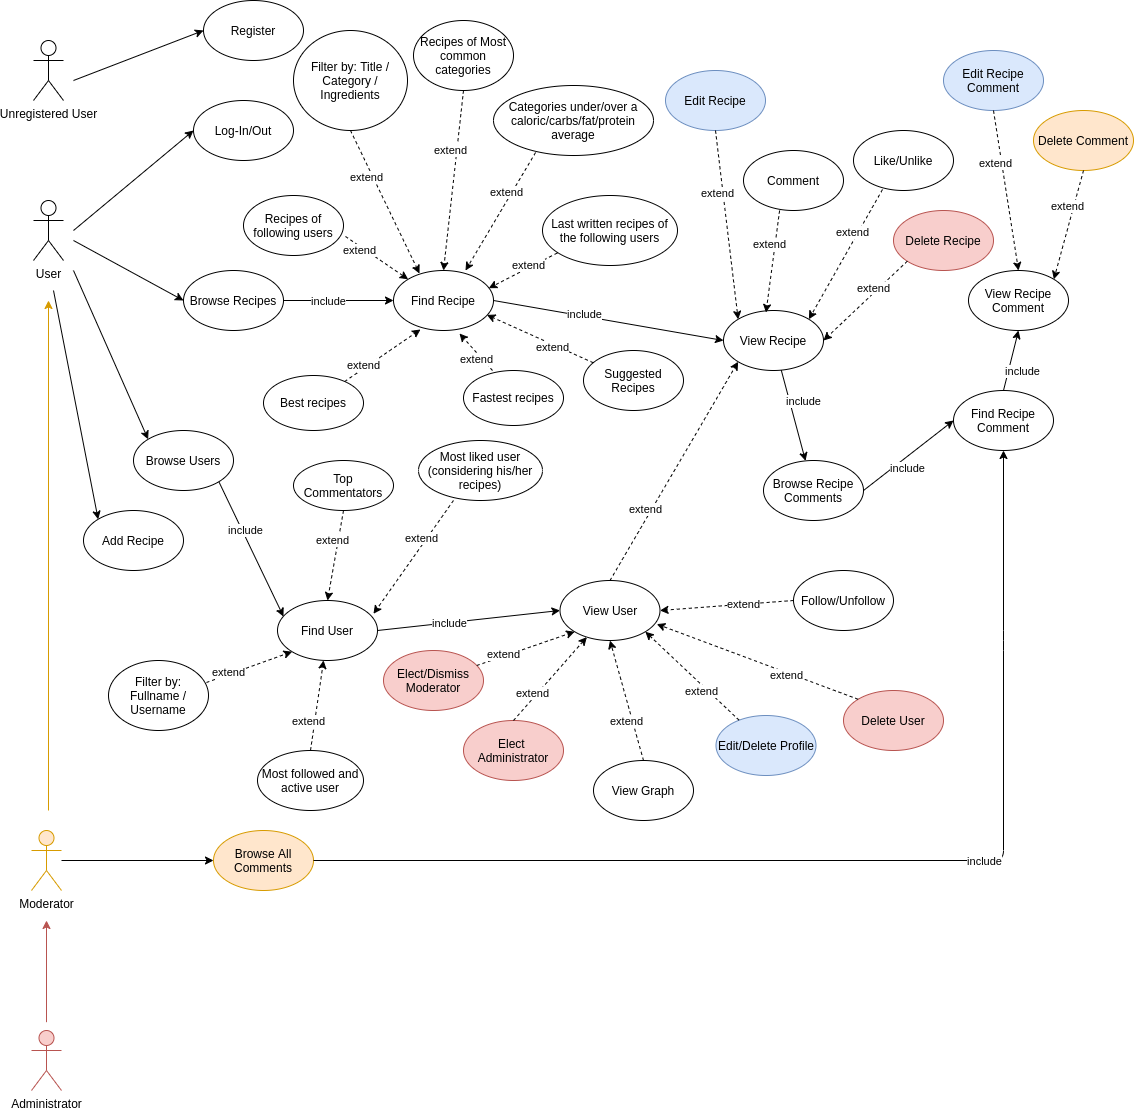
\includegraphics[scale=0.5]{img/UseCaseDiagram.png}
	\caption{Use Case Diagram}
\end{figure}
\section{UML Class Diagram}
\section{Data Model}
\subsection{DocumentDB}
\subsection{GraphDB}
\section{Distributed Database Design}
\subsection{Replicas}
\subsection{Sharding}
\section{Software Architecture}


\chapter{Implementation and Test}
\section{Main Modules}
\section{Main Packages and Classes}
\section{Most Relevant Queries}
\subsection{MongoDB}
\subsection{Neo4J}
\section{Unit Test}
\section{Tests and Statistical Analysis}

\chapter{User Manual}
\end{document}